% Metódy inžinierskej práce

\documentclass[10pt,twocolumn,twoside,slovak,a4paper]{coursepaper} % Pridany parameter twocolumn

\usepackage[slovak]{babel}
\usepackage[IL2]{fontenc} % lepšia sadzba písmena Ľ než v T1
\usepackage[utf8]{inputenc}
\usepackage{graphicx}
\usepackage{wrapfig} % Pridané pre obtekanie textu okolo loga FIIT
\usepackage{amsmath} % Pridané pre matice a dlhé viacriadkové vzorce
\usepackage{url} % príkaz \url na formátovanie URL
\usepackage{hyperref} % odkazy v texte budú aktívne

\usepackage{cite}
\usepackage{todonotes}

\pagestyle{headings}

\title{Súčasné trendy vo vývoji automatizovaných systémov s využitím asynchrónneho programovania v jazyku Python\thanks{Semestrálny projekt v predmete Metódy inžinierskej práce, ak. rok 2026/27, vedenie: Richard Marko}}

\author{Oleksii Kovalevskyi\\[2pt]
	{\small Slovenská technická univerzita v Bratislave}\\
	{\small Fakulta informatiky a informačných technológií}\\
	{\small \texttt{xkovalevskyi@stuba.sk}}
	}

\date{\small 28. september 2026}

\begin{document}
\maketitle

\begin{abstract}
Tento článok poskytuje prehľad súčasného stavu v oblasti vývoja automatizovaných softvérových botov s využitím asynchrónneho programovania. Zameriava sa na moderné prístupy a knižnice v jazyku Python, ako sú aiogram a apscheduler, ich architektúru, výhody a úskalia pri nasadzovaní v reálnych aplikáciách. Cielom je zosumarizovať dostupné riešenia a porovnať ich efektivitu.
\end{abstract}


\section{Úvod}
\begin{wrapfigure}{r}{0.3\textwidth}
    \centering
    
\includegraphics[width=0.25\textwidth]{STU-FIIT-anch.png}
    \caption{Logo FIIT STU}
\end{wrapfigure}
Asynchrónne programovanie v jazyku Python predstavuje moderný prístup k vývoju softvéru, ktorý umožňuje efektívne spracovanie veľkého množstva paralelných úloh. Tento článok sa zameriava na knižnice ako aiogram a apscheduler. Použitie takýchto nástrojov je kľúčové pre tvorbu rýchlych a škálovateľných automatizovaných botov. Tento odsek bol doplnený tak, aby bolo viditeľné plynulé obtekanie textu okolo vloženého plávajúceho loga fakulty, presne podľa požiadaviek cvičenia.

\section{Prehľad architektúry asynchrónnych systémov}
V tejto časti analyzujeme základnú štruktúru bota. Na nasledujúcich diagramoch môžeme vidieť rozdelenie komponentov a tok spracovania správ. Nasledujúce dva diagramy sú umiestnené vedľa seba.

\begin{figure}[h]
    \centering
    \begin{minipage}{0.45\textwidth}
        \centering
        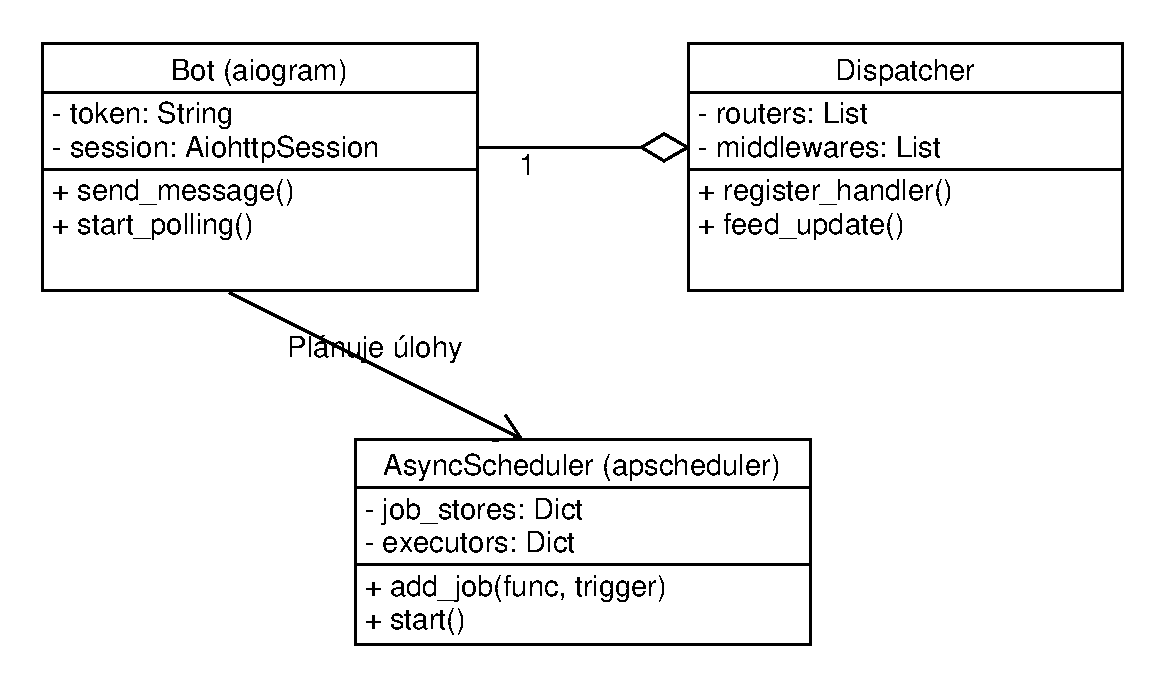
\includegraphics[width=\textwidth]{diagram1.pdf}
        \caption{Architektúra Python bota}
    \end{minipage}\hfill
    \begin{minipage}{0.45\textwidth}
        \centering
        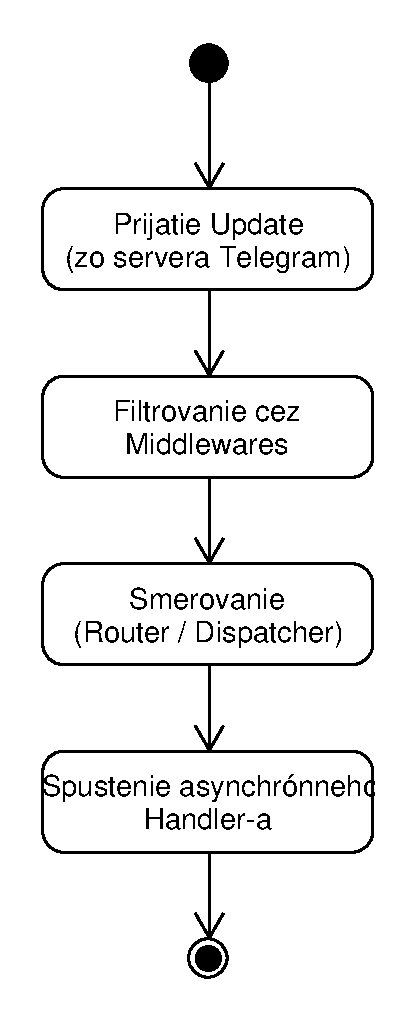
\includegraphics[width=\textwidth]{diagram2.pdf}
        \caption{Spracovanie updatov}
    \end{minipage}
\end{figure}

\section{Analýza moderných nástrojov v jazyku Python}
Knižnice aiogram a apscheduler poskytujú robustné API pre vývojárov. Vďaka event-loopu v Pythone nedochádza k blokovaniu hlavného vlákna pri čakaní na odpoveď zo servera Telegramu. Pre detailný pohľad uvádzame široký diagram prekrývajúci oba stĺpce.

\begin{figure*}[h!]
    \centering
    % Úprava veľkosti na 80% šírky strany
    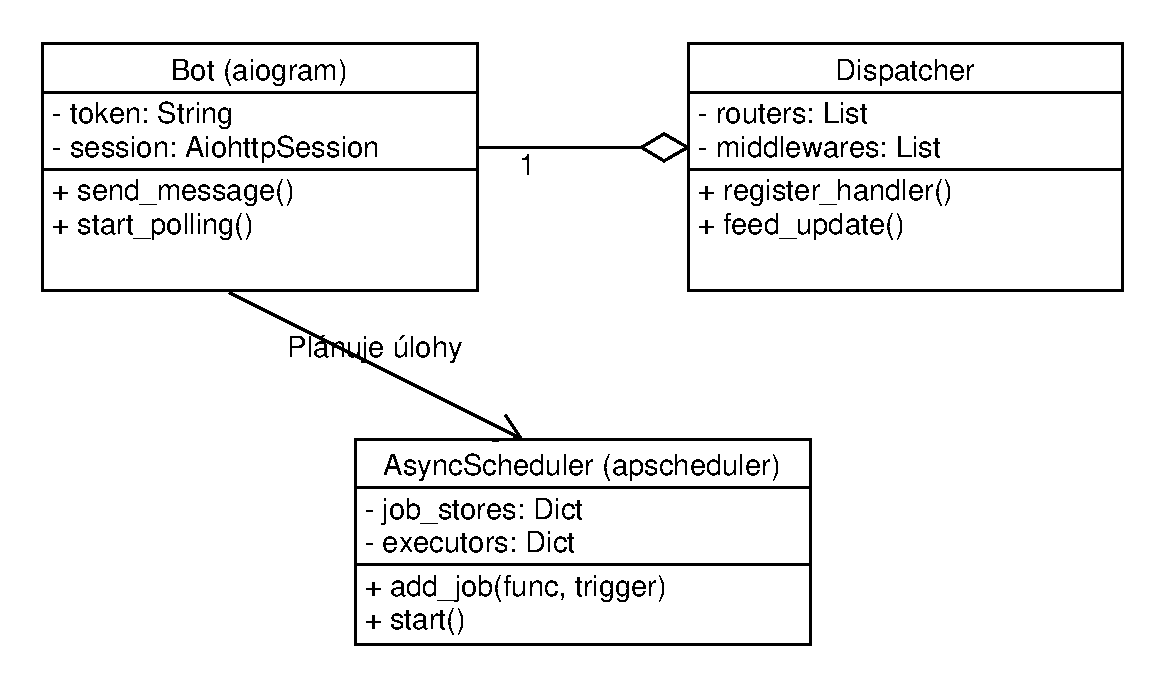
\includegraphics[width=0.8\textwidth, angle=0]{diagram1.pdf} 
    \caption{Celkový pohľad na asynchrónny systém prekrývajúci obidva stĺpce}
\end{figure*}

\section{Porovnanie a zhodnotenie prístupov}
Pri porovnávaní výkonnosti asynchrónnych systémov môžeme stavy jednotlivých taskov (úloh) vizualizovať pomocou stavovej matice s rozmerom 5x4:

\[
\begin{bmatrix}
task_{11} & task_{12} & task_{13} & task_{14} \\
task_{21} & task_{22} & task_{23} & task_{24} \\
task_{31} & task_{32} & task_{33} & task_{34} \\
task_{41} & task_{42} & task_{43} & task_{44} \\
task_{51} & task_{52} & task_{53} & task_{54}
\end{bmatrix}
\]

Na výpočet celkovej časovej zložitosti a odozvy systému pri veľkom zaťažení (napríklad pri plánovaní stoviek úloh) používame nasledujúci rozvoj, ktorý svojou dĺžkou presahuje šírku jedného stĺpca dokumentu, a preto je zalomený do viacerých riadkov:

\begin{multline}
T_{total} = t_{init} + \sum_{i=1}^{n} (p_i \cdot w_i) + c_{db} + c_{api} + c_{cache} + \\
+ \delta_{net1} + \delta_{net2} + \delta_{net3} + \delta_{net4} + \delta_{net5} + \mathcal{O}(N \log N)
\end{multline}

\section{Záver}
Asynchrónne systémy v Pythone predstavujú efektívne riešenie pre moderné aplikácie. V ďalšej práci na prehľadovom článku sa zameriame na hlbšiu optimalizáciu a možnosti nasadenia v produkčnom prostredí s ohľadom na dostupné zdroje.

\bibliography{literatura}
\bibliographystyle{alpha}
\end{document}